\chapter{Evaluation}

Dieses Kapitel widmet sich einer umfassenden Analyse der Relevanz und Effektivität des GReQL Converters als innovatives
Werkzeug. Spezifisch zielt diese Abschnitt darauf ab, die grundlegende Frage zu beantworten, ob dieses Instrument
tatsächlich im akademischen und pädagogischen Kontext nützlich ist. Um dieses Ziel zu erreichen, ist es von größter
Wichtigkeit, eine systematische Herangehensweise zu verfolgen, die die Anwendung verschiedener Bewertungsmethoden
beinhaltet, um die Vorzüge und Effektivität des GReQL Converters nachzuweisen. Dieses Kapitel behandelt ausführlich die
angewandten Ansätze zur Prüfung des GReQL Converters, die Datensammlungsmethoden und die durchgeführten Analysen zur
Messung seiner Nützlichkeit. Letztendlich geht es darum, empirisch festzustellen, ob dieses Werkzeug konkrete Vorteile
und einen signifikanten Mehrwert für Lehrende und Lernende bietet.

\section{Erreichte Ziele}

Die Untersuchung der Effizienz und Funktionalität des GReQL Converters als Instrument zur Extraktion relevanter
GReQL-Regeln aus einer UML-Diagrammannotation, die mittels PlantText zur Evaluation von UML-Diagrammen erstellt wurde,
stellt eine essenzielle Fragestellung dar, welche eine systematische und tiefgehende Herangehensweise erfordert. In dem
Implementierungskapitel (siehe ~\ref{ch:implementierung}) wurden diverse Regeln vorgestellt, begleitet von einer detaillierten Erläuterung des
spezifischen Extraktionsprozesses für jede dieser Regeldefinitionen. Gleichwohl erwies sich eine umfassende Testphase
als unverzichtbar, um eine eingehende Evaluierung der Leistungsfähigkeit jeder einzelnen Regel zu ermöglichen.

Zur Durchführung dieser Evaluierungen wurden verschiedene Testverfahren appliziert, welche eine Vielzahl von Szenarien
und Variationen abdeckten, mit dem Ziel, die Effizienz der durch den GReQL Converter generierten Regeldefinitionen
im Detail zu beurteilen. Der Testprozess kann in vier diskrete Schritte unterteilt werden:

\begin{enumerate}
    \item Initiale Generierung eines Diagramms mithilfe von PlantText, wobei dieses Diagramm gezielt konzipiert wurde,
um die spezifischen Merkmale der zu evaluierenden Regel zu inkorporieren. Zum Beispiel wurde ein Diagramm erstellt,
welches eine Aggregation zwischen zwei Klassen darstellte, um eine Regel zur Aggregation zu prüfen.
    \item Erstellung eines Evaluationsdiagramms (welches in diesem Kontext mittels BOUML modellisiert wurde), welches von
den generierten Regeldefinitionen bewertet werden sollte.
    \item Extraktion der verschiedenen Regeldefinitionen aus dem PlantText-Code.
    \item Evaluierung mithilfe der GReQL-Engine von JACK, um festzustellen, ob die Regeldefinitionen die Aggregation
im Diagramm effektiv erkannt haben.
\end{enumerate}

Parallelen dazu wurde besonderes Augenmerk auf die Identifikation von falsch positiven (False Positiv) Ergebnissen
gerichtet, welche den Eindruck einer korrekten Funktionsweise des Werkzeugs erwecken könnten, obwohl dem nicht so ist.
Hierzu wurde eine sorgfältige Analyse des generierten Codes durchgeführt, und die Protokolle der GReQL-Engine wurden
überprüft, um die präzise Identifikation der Aggregationsregel sicherzustellen. Es sei hervorgehoben, dass dieser
gewissenhafte Überprüfungsprozess in systematischer Weise auf alle vorab definierten Regeldefinitionen der
Implementierungsphase angewandt wurde.

Im Anschluss an die individuelle Prüfung jeder Regeldefinition erfolgte eine Evaluierung anhand zunehmend komplexerer
Diagramme. Das Ziel bestand darin, mehrere Funktionen simultan zu bewerten und zu ermitteln, ob die Existenz mehrerer
Verknüpfungen zwischen verschiedenen Elementen im Diagramm spezifische Regeldefinitionen nicht beeinträchtigte. Die
Bedingungen, die zu potenziellen Konflikten führen könnten, wurden somit eingehend untersucht, und der GReQL Converter
wurde bei jeder Fehlererkennung oder -identifikation angepasst, um seine Effizienz zu steigern.

In einem darauffolgenden Schritt wurden verschiedene gängige Übungen zu UML-Diagrammen selektiert, um die akademische
Leistung der Studierenden an der Universität zu evaluieren. Unter diesen Übungen findet sich das Diagramm ``Mendelssohn
\& Sohn Maschinenbau GmbH'', welches im Rahmen des Kurses ``Einführung in die Unified Modeling Language'' an der
Universität Potsdam zum Einsatz kam (siehe~\ref{fig:bau_gmbh}). Dieses spezifische Diagramm weist signifikante
Ähnlichkeiten zu den traditionellen Modellen auf, die in universitären Prüfungskontexten verwendet werden, wodurch es
sich als exemplarisches Testobjekt zur Ermittlung der Leistungsfähigkeit des GReQL Converters erweist.

Zu diesem Ziel wurde das Musterdiagramm, das als Repräsentation der Übungsvorlage diente, mittels des Werkzeugs
BOUML modelliert. Anschließend erfolgte die Extraktion der XMI-Datei, welche als Bewertungsinstrument diente. Parallel
dazu wurde die Anwendung von PlantText zur Erstellung der Musterdiagrammvorlage in Erwägung gezogen, wobei der GReQL
Converter im Anschluss dazu verwendet wurde, um die Regeln gemäß dem vorab beschriebenen Verfahren formal zu erfassen.
Subsequent zur Extraktion der Regeldefinitionen und der willkürlichen Punktevergabe für jede einzelne Regel, unterzog
man diese Regeldefinitionen einer Evaluation im Rahmen des GReQL-Motors von JACK.

Hervorzuheben ist, dass für ein mittelkomplexes Diagramm wie das genannte insgesamt \textbf{82 GReQL-Regeln} generiert
wurden. Nach abschließenden Tests ergab sich, dass der GReQL-Motor eine Erfolgsrate von 100\% aufwies, was auf die
korrekte Funktionalität der erzeugten Regeldefinitionen hinweist. Dieser Erfolg illustriert eindrucksvoll die Befähigung
des GReQL Converters zur effektiven Evaluierung von UML-Diagrammen, insbesondere jener von erhöhter Komplexität.

\begin{figure}[h]
    \centering
    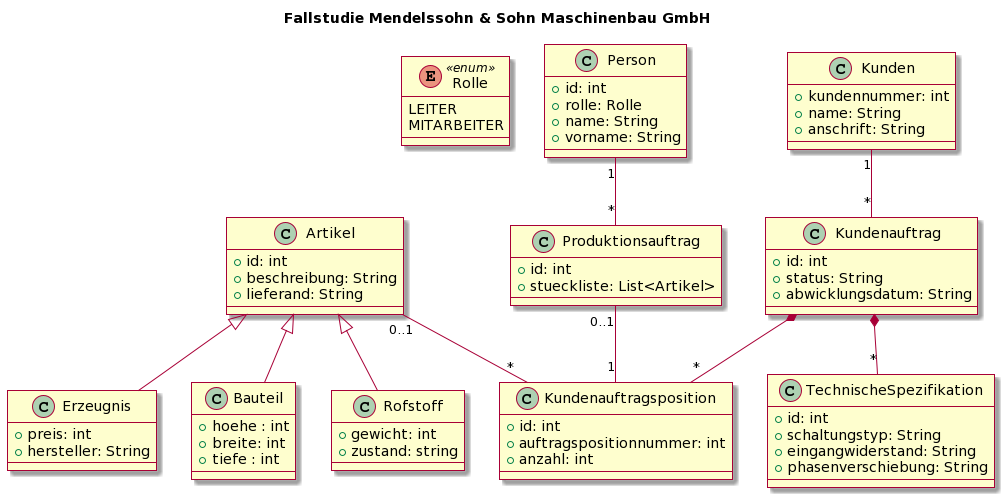
\includegraphics[width=16cm]{images/bau_gmbh_plantText}
    \caption{Fallstudie UML - Klassendiagramm}
    \label{fig:bau_gmbh}
\end{figure}

In Bezug auf die Leistungen, die dem GReQL Converter zugeschrieben werden können, lassen sich folgende Punkte
feststellen:

\begin{enumerate}
    \item Der GReQL Converter ermöglicht die umfassende Bewertung eines Diagramms. Im vorherigen Beispiel ermöglichte er
die Generierung von 82 Regeln, eine Aufgabe, die besonders mühsam und fehleranfällig wäre, wenn sie manuell von einem
Lehrer durchgeführt würde.
    \item Der GReQL Converter führt Bewertungen äußerst präzise durch und verhindert somit potenzielle Fehler, die
Lehrer bei manuellen Bewertungen begehen könnten.
    \item Der GReQL Converter verhindert Fehler in Bezug auf die Syntax und Formulierung von Regeln, insbesondere
solche, die bereits vom Tool definiert sind, was den Benutzer von Sorgen in Bezug auf diese Aspekte entlastet.
    \item Darüber hinaus ist eine direkte Interaktion mit dem GReQL-Code nicht mehr erforderlich, da der Benutzer die
Regeln problemlos ändern kann, indem er die generierten Objekte nach dem Schritt der syntaktischen Analyse verwendet,
was den Bearbeitungsprozess vereinfacht.
    \item Der GReQL Converter erleichtert erheblich das Verständnis des GReQL-Codes, indem er klaren, lesbaren und
zugänglichen Code generiert, was es Dritten ermöglicht, seine Funktionsweise zu verstehen und bei Bedarf Änderungen
vorzunehmen.
    \item Darüber hinaus berücksichtigt das Design des Tools die Vielfalt grundlegender Varianten in UML-Diagrammen,
was seine Vielseitigkeit und Anpassungsfähigkeit stärkt.
\end{enumerate}

Wenn man diese Vorteile mit den in Teil drei aufgeführten Problemen vergleicht, die die
Problemanalyse (siehe~\ref{ch:problemanalyse}) behandelten, steht außer Frage, dass der GReQL Converter seine Rolle als
Hilfsmittel bei der Erstellung von GReQL-Code für die Bewertung von Klassendiagrammen erfüllt und Lehrern erheblich
Zeit spart. Im nächsten Abschnitt wird eine Studie durchgeführt, um zu ermitteln, ob Lehrende diese Ansicht teilen.

\section{Interview zur Bewertung des GReQL Converters}
todo - write something here